\documentclass[10pt,twocolumn,letterpaper]{article}

\usepackage{cvpr}
\usepackage[utf8]{inputenc}
\usepackage{gensymb}
\usepackage{graphicx}
\usepackage{caption}
\usepackage{subcaption}
\usepackage{mathtools}
\graphicspath{ {report3-imgs/} }
\usepackage{float}
\PassOptionsToPackage{hyphens}{url}\usepackage{hyperref}

\cvprfinalcopy
\def\cvprPaperID{a1700831}


% begin of document
\begin{document}
\title{Assignment 3 - Method for Generating Image Descriptions}
\author{Yuanzhong Xia\\
University of Adelaide\\
SA, Australia\\
{\tt\small a1700831@student.adelaide.edu.au}
}
\maketitle

% abstract
\begin{abstract}
% TODO: abstract
\end{abstract}

% content
\section{The Problem}
The problem is to give a sentence in natural language of the description for an input image.

This problem is very typical, because it is very challenging that it transforms information from ``image'' type to ``text'' type.
The input image should firstly be understood by the artificial intelligence,
then it should be able to output a descriptive text to tell what the input image shows.

The relative applications can be various, like: helping human to automatically pointing out the objectives and events in a massive number of images,
and helping visually impaired people to see. But the most difficult challenge is not only understanding both image and natural language,
but also the information transformation.


\section{Background}
Before this paper by Karpathy \textit{et al.} \cite{origin}. There are plenty of researches challenging this problem,
which can be mainly divided into three types.

\subsection{Image annotating strategy}
A typical way to annotate images is classifying or tagging images \cite{everingham}, \cite{russakovsky}.
In a fixed word dictionary, the image tagging can be more meaningful because unwanted words are discarded at the beginning.
The weakness is that the words in dictionary are often not rich enough.

Barnard \textit{et al.} \cite{barnard} and Socher \textit{et al.} \cite{socher}'s researches uses the images,
whose segments are annotated instead the whole image, as the training input data.
That helps the object recognition process, but requires more human works.

Gould \textit{et al.}'s research \cite {gould} used a method to extract scene feature,
so that the relationships between objects and the scene can be easily connected.
However, their work was focusing on labelling the scene, while the proposed method is used to
generate richer and high-level descriptions of the image, no matter what the scene labels are.


\subsection{Description generating strategy}
Methods from Kulkarni \textit{et al.} \cite{kulkarni} limit the resulting sentence number in one;
whereas this paper's authors think that manual restriction is not necessary and it reduces the artificial intelligence's creativity.

Matuszek \textit{et al.} \cite{matuszek} used grounding dependency tree relations which arrange words in a vector space.
The vector space would limit the results to some extend, like the sentence length, etc.


\subsection{Connecting between images and natural language strategy}
The earlier pioneering methods by Farhadi \textit{et al.} \cite{farhadi} hard-coded visual concepts and explicitly defined sentence.
Images objects or scenes are pre-defined, then marked images are learnt by the system so that the system can recognize defined things.
However, these methods limited the language variety and required much human works to define the connecting between language words and the images first.

Now, pre-trained image/word vectors are quite popular.
For images, ImageNet \cite{imagenet} is a very popular pre-trained image recognition model;
for words, previous works \cite{bengio}, \cite{socher2}, \cite{mikolov} mentioned the pre-trained word vectors
to obtain low-dimensional representations of words.
Additionally, in the original paper, the authors use these pre-trained models as well.


\section{Algorithm Description}
Unlike the previous approaches, the proposed method in Karpathy \textit{et al.}'s paper is to let the artificial neural networks
learn the pattern between images and sentences automatically.
Therefore there is no limitation for this method literally,
because the training data can be arbitrary, and the model thus will be adjusted by the training data.

\subsection{Training}
The overview of training algorithm steps is as follows,
\begin{enumerate}
    \item Prepare the training images and corresponding sentences;
          \textit{(datasets mentioned in the paper are flickr8k, flickr30k and MSCOCO,
          and sometimes each image has multiple descriptive sentences.)}
    \item Extract 4096 dimensional features vector using pre-trained CNN model on ImageNet \cite{imagenet};
          \textit{(this model contains objects of 200 classes, which is described in ImageNet Detection Challenge \cite{inch}.)}
    \item Train the multimodal RNN sentence generator which takes a word to predict the next following word, by passing the words one by one and the image feature matrix;
          \textit{(``START'' and ``END'' are two special tokens in this RNN, and the words are sent to the RNN one by one.)}
\end{enumerate}
% TODO: how to tag more effectively (+5 times selected)

\subsection{Predicting}
To predict an image:
\begin{enumerate}
    \item Prepare testing images;
    \item Extract 4096 dimensional features vector using pre-trained CNN model on ImageNet;
          \textit{(same as training.)}
    \item Generate description from multimodal RNN by setting ``START'' token and image representation matrix;
          \textit{(until ``END'' is generated, the description is finished generating.)}
\end{enumerate}

\subsection{Benchmark}
The original paper also mentions the methods for predicting region text information (to mark the regions like Figure \ref{fig:region}):
\begin{enumerate}
    \item When having the image feature vector;
    \item Calculate the image representation matrix using top 19 detected known objects by the dot product between feature vector and a parameter matrix $W_{m}$;
          \textit{(the representation matrix in the paper is in the shape of 20 $h$-dimensional vectors, thus this is the recognizable resolution.)}
    \item Calculate the sentence representation vector using Bidirectional Recurrent Neural Network (BRNN) \cite{brnn};
          \textit{(each input sentence sequence is transformed into a $h$ dimensional vector;
          during the calculation, BRNN takes two directional word relations to maintain a context;
          then, a word vocabulary is built automatically by the methods from Mikolov et al. \cite{mikolov}.)}
    \item Calculate image-sentence score by dot product between sentence representation vector and image representation matrix and a $max$ operation;
          \textit{(this method is proved by their previous work \cite{karpathy},
          and the resulting image-sentence score is actually calculated by the image region-word score,
          with the dimension of 20.)}
    \item Align words with corresponding regions in Markov Random Field (MRF) to get an annotated region set;
          \textit{(each region has multiple words aligned with;
          to find the best alignment, the authors use dynamic programming by Viterbi et al. \cite{viterbi}.)}
\end{enumerate}

The ``image-sentence score'' is the benchmark value, and the experiments from the original paper use this score ranking for comparisons.

\begin{figure*}
    \begin{center}
        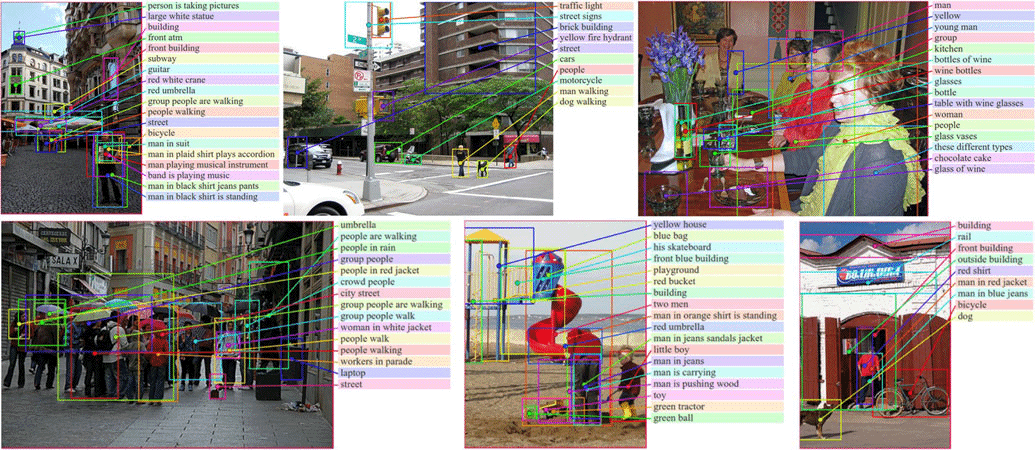
\includegraphics[width=0.9\textwidth]{region.png}
    \end{center}
    \caption{The region prediction from the original paper. This figure is the Fig. 9 in original paper.}
    \label{fig:region}
\end{figure*}


\section{Hypothesis and limitations}
\subsection{Two model issue}
The proposed methods in original paper use two models for the final prediction:
the object recognision model and description generator model.
Two models are trained with different datasets.

Thus, my hypothesis is,
\begin{enumerate}
    \item the objects which are in the first training dataset but not in the second dataset
          will take an unnecessary weight in the first model;
    \item the objects which are not in the first training dataset but in the sencond dataset
          will not be detected.
\end{enumerate}

In the original paper, the first model is pre-trained for object recognision by ImageNet \cite{imagenet}.
This is a tree-based model (database) containing 5247 categories of objects, and builded by around 50 million images.
And the original paper uses 200 categories from The ImageNet Detection Challenge \cite{inch}.
Given the input image, the nearest neighbor methods can vote and return the recognized object.
However, the tree nodes are taken by unused objects, thus the the rate of mis-recognision increases, which supports my first statement.

For the second statement, the image representation matrix is calculated as
$$v = W_{m} \left [ CNN_{\theta_{c}}(I_{b}) \right ] + b_{m}$$
the resulting matrix from $CNN$ will have un-detected cells filling with $0$.
And therefore, after the dot product with sentence representation vector
$$S_{kl} = \sum_{t \in texts} max_{i \in cells}(v_{i}^{T}s_{t})$$
where $v_{i}^{T}$ is the image representation matrix and $s_{t}$ is the representation matrix.
The un-detected words will thus result in $0$.
Hence, those objects not in the recognision model (first dataset) cannot be detected even if they are in the secodn dataset.


\subsection{Resolution issue}
The image feature size is fixed to 4096 dimensions in the original paper.
My hypothesis is that, if the image is too larger than its inside objects, the objects cannot even be recognized.

In the original paper, the feature set of an image is expressed in a 4096 dimension vector.
If the image is super large, and the objects cannot be effectively detected and stored in the feature vector,
the image will be difficult to be summarized correctly. An experiment is mentioned in Section \ref{sec:hs}.


\subsection{Unexpected object issue}
My hypothesis is that unexpected objects will result in unexpected sentences.

This is a common machine learning issue, but with different apprearance on results.
I guess the results will still be a complete sentence even when there is nothing in the input image,
because the structure of RNN is building sentence from the beginning to the end.
The experiment is discussed in Section \ref{sec:uo}.


\subsection{Language grammar issue}
My hypothesis is that it learns from non-systematic sentences, thus there must be grammar errors leading to a different meaning.

% TODO: 1001773457_577c3a7d70.jpg#0	A black dog and a spotted dog are fighting
Due to the training methods in the original paper,



\section{Experiments}
% TODO: details set up

% TODO: log prob, but how is it calculated

% TODO; benchmark on flickr8k's 1k

\subsection{Experiments for hypothesis}
% TODO benchmark on hypothesis
\subsubsection{High resolution experiment} \label{sec:hs}

\subsubsection{Unexpected object experiment} \label{sec:uo}

\subsubsection{Language grammar experiment} \label{sec:lg}





\section{Conclusion}


% Bibliography
\begin{thebibliography}{99}
\bibitem {origin}
A. Karpathy and L. Fei-Fei, Deep visual-semantic alignments for generating image descriptions,
In \textit{Proceedings of the IEEE Conference on Computer Vision and Pattern Recognition}, pp. 3128-3137, 2015.

\bibitem {kulkarni}
G. Kulkarni, et al., Baby talk: Understanding and generating simple image descriptions,
In \textit{Proc. IEEE Conf. Comput. Vis. Pattern Recog.}, pp. 1601-1608, 2011.

\bibitem {farhadi}
A. Farhadi, et al., Every picture tells a story: Generating sentences from images,
In \textit{Proc. 11th Eur. Conf. Comput. Vis.}, pp. 15-29, 2010.

\bibitem {everingham}
M. Everingham, L. Van Gool, C. K. I. Williams, J. Winn, and A. Zisserman, The Pascal visual object classes (VOC) challenge,
In \textit{Int. J. Comput. Vis.}, vol. 88, no. 2, pp. 303–338, 2010.

\bibitem {russakovsky}
O. Russakovsky, et al., Imagenet large scale visual recognition challenge,
In \textit{Int. J. Comput. Vis.}, vol. 115, no. 3, pp. 211–252, 2015.

\bibitem {barnard}
K. Barnard, P. Duygulu, D. Forsyth, N. De Freitas, D. M. Blei, and M. I. Jordan, Matching words and pictures,
In \textit{J. Mach. Learn. Res.}, vol. 3, pp. 1107–1135, 2003.

\bibitem {socher}
R. Socher and L. Fei-Fei, Connecting modalities: Semi-supervised segmentation and annotation of images using unaligned text corpora,
In \textit{Proc. IEEE Conf. Comput. Vis. Pattern Recog.}, pp. 966–973, 2010.

\bibitem {gould}
S. Gould, R. Fulton, and D. Koller, Decomposing a scene into geometric and semantically consistent regions,
In \textit{Proc. IEEE 12th Int. Conf. Comput. Vis.}, pp. 1–8, 2009.

\bibitem {matuszek}
C. Matuszek, N. FitzGerald, L. Zettlemoyer, L. Bo, and D. Fox, A joint model of language and perception for grounded attribute learning,
In \textit{Proc. 29th Int. Conf. Mach. Learn.}, pp. 1671–1678, 2012.

\bibitem {bengio}
Y. Bengio, H. Schwenk, J.-S. Senecal, F. Morin, and J.-L. Gauvain, Neural probabilistic language models,
In \textit{Innovations in Machine Learning. Berlin, Germany}, 2006.

\bibitem {socher2}
R. Socher, J. Pennington, and C. Manning, Glove: Global vectors for word representation,
In \textit{Proc. Empirical Methods Natural Language Process.}, pp. 1532–1543, 2014.

\bibitem {mikolov}
T. Mikolov, I. Sutskever, K. Chen, G. S. Corrado, and J. Dean, Distributed representations of words and phrases and their compositionality,
In \textit{Proc. Advances Neural Inf. Process. Syst.}, pp. 3111–3119, 2013.

\bibitem {imagenet}
J. Deng, W. Dong, R. Socher, L.-J. Li, K. Li, and L. Fei-Fei, ImageNet: A large-scale hierarchical image database,
In \textit{Proc. IEEE Conf. Comput. Vis. Pattern Recog.}, pp. 248–255, 2009.

\bibitem {inch}
O. Russakovsky, et al., Imagenet large scale visual recognition challenge,
In \textit{Int. J. Comput. Vis.}, vol. 115, no. 3, pp. 211–252, 2015.

\bibitem {brnn}
M. Schuster and K. K. Paliwal, Bidirectional recurrent neural networks,
In \textit{IEEE Trans. Signal Process.}, vol. 45, no. 11, pp. 2673–2681, 1997.

\bibitem {karpathy}
A. Karpathy, A. Joulin, and F. F. F. Li, Deep fragment embeddings for bidirectional image sentence mapping,
In \textit{Proc. Advances Neural Inf. Process. Syst.}, pp. 1889–1897, 2014.

\bibitem {viterbi}
A. J. Viterbi, Error bounds for convolutional codes and an asymptotically optimum decoding algorithm,
in \textit{IEEE Trans. Inf. Theory}, vol. TIT-13, no. 2, pp. 260–269, 1967.

\end{thebibliography}

\end{document}
